\documentclass[twoside]{book}

% Packages required by doxygen
\usepackage{fixltx2e}
\usepackage{calc}
\usepackage{doxygen}
\usepackage[export]{adjustbox} % also loads graphicx
\usepackage{graphicx}
\usepackage[utf8]{inputenc}
\usepackage{makeidx}
\usepackage{multicol}
\usepackage{multirow}
\PassOptionsToPackage{warn}{textcomp}
\usepackage{textcomp}
\usepackage[nointegrals]{wasysym}
\usepackage[table]{xcolor}

% Font selection
\usepackage[T1]{fontenc}
\usepackage[scaled=.90]{helvet}
\usepackage{courier}
\usepackage{amssymb}
\usepackage{sectsty}
\renewcommand{\familydefault}{\sfdefault}
\allsectionsfont{%
  \fontseries{bc}\selectfont%
  \color{darkgray}%
}
\renewcommand{\DoxyLabelFont}{%
  \fontseries{bc}\selectfont%
  \color{darkgray}%
}
\newcommand{\+}{\discretionary{\mbox{\scriptsize$\hookleftarrow$}}{}{}}

% Page & text layout
\usepackage{geometry}
\geometry{%
  a4paper,%
  top=2.5cm,%
  bottom=2.5cm,%
  left=2.5cm,%
  right=2.5cm%
}
\tolerance=750
\hfuzz=15pt
\hbadness=750
\setlength{\emergencystretch}{15pt}
\setlength{\parindent}{0cm}
\setlength{\parskip}{3ex plus 2ex minus 2ex}
\makeatletter
\renewcommand{\paragraph}{%
  \@startsection{paragraph}{4}{0ex}{-1.0ex}{1.0ex}{%
    \normalfont\normalsize\bfseries\SS@parafont%
  }%
}
\renewcommand{\subparagraph}{%
  \@startsection{subparagraph}{5}{0ex}{-1.0ex}{1.0ex}{%
    \normalfont\normalsize\bfseries\SS@subparafont%
  }%
}
\makeatother

% Headers & footers
\usepackage{fancyhdr}
\pagestyle{fancyplain}
\fancyhead[LE]{\fancyplain{}{\bfseries\thepage}}
\fancyhead[CE]{\fancyplain{}{}}
\fancyhead[RE]{\fancyplain{}{\bfseries\leftmark}}
\fancyhead[LO]{\fancyplain{}{\bfseries\rightmark}}
\fancyhead[CO]{\fancyplain{}{}}
\fancyhead[RO]{\fancyplain{}{\bfseries\thepage}}
\fancyfoot[LE]{\fancyplain{}{}}
\fancyfoot[CE]{\fancyplain{}{}}
\fancyfoot[RE]{\fancyplain{}{\bfseries\scriptsize Generated by Doxygen }}
\fancyfoot[LO]{\fancyplain{}{\bfseries\scriptsize Generated by Doxygen }}
\fancyfoot[CO]{\fancyplain{}{}}
\fancyfoot[RO]{\fancyplain{}{}}
\renewcommand{\footrulewidth}{0.4pt}
\renewcommand{\chaptermark}[1]{%
  \markboth{#1}{}%
}
\renewcommand{\sectionmark}[1]{%
  \markright{\thesection\ #1}%
}

% Indices & bibliography
\usepackage{natbib}
\usepackage[titles]{tocloft}
\setcounter{tocdepth}{3}
\setcounter{secnumdepth}{5}
\makeindex

% Hyperlinks (required, but should be loaded last)
\usepackage{ifpdf}
\ifpdf
  \usepackage[pdftex,pagebackref=true]{hyperref}
\else
  \usepackage[ps2pdf,pagebackref=true]{hyperref}
\fi
\hypersetup{%
  colorlinks=true,%
  linkcolor=blue,%
  citecolor=blue,%
  unicode%
}

% Custom commands
\newcommand{\clearemptydoublepage}{%
  \newpage{\pagestyle{empty}\cleardoublepage}%
}

\usepackage{caption}
\captionsetup{labelsep=space,justification=centering,font={bf},singlelinecheck=off,skip=4pt,position=top}

%===== C O N T E N T S =====

\begin{document}

% Titlepage & ToC
\hypersetup{pageanchor=false,
             bookmarksnumbered=true,
             pdfencoding=unicode
            }
\pagenumbering{alph}
\begin{titlepage}
\vspace*{7cm}
\begin{center}%
{\Large My Project }\\
\vspace*{1cm}
{\large Generated by Doxygen 1.8.13}\\
\end{center}
\end{titlepage}
\clearemptydoublepage
\pagenumbering{roman}
\tableofcontents
\clearemptydoublepage
\pagenumbering{arabic}
\hypersetup{pageanchor=true}

%--- Begin generated contents ---
\chapter{Class Index}
\section{Class List}
Here are the classes, structs, unions and interfaces with brief descriptions\+:\begin{DoxyCompactList}
\item\contentsline{section}{\hyperlink{structHeap}{Heap} }{\pageref{structHeap}}{}
\item\contentsline{section}{\hyperlink{structNode}{Node} }{\pageref{structNode}}{}
\end{DoxyCompactList}

\chapter{File Index}
\section{File List}
Here is a list of all documented files with brief descriptions\+:\begin{DoxyCompactList}
\item\contentsline{section}{include/\hyperlink{car_8h}{car.\+h} \\*File containing the function definitions needed for car struct }{\pageref{car_8h}}{}
\end{DoxyCompactList}

\chapter{Class Documentation}
\hypertarget{structHeap}{}\section{Heap Struct Reference}
\label{structHeap}\index{Heap@{Heap}}


{\ttfamily \#include $<$heaphelper.\+h$>$}



Collaboration diagram for Heap\+:\nopagebreak
\begin{figure}[H]
\begin{center}
\leavevmode
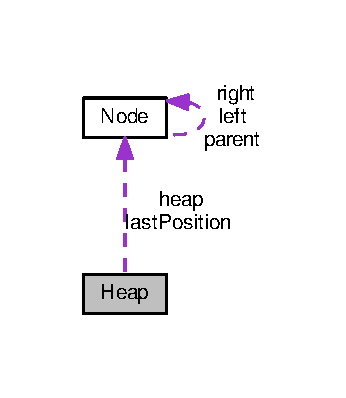
\includegraphics[width=166pt]{structHeap__coll__graph}
\end{center}
\end{figure}
\subsection*{Public Attributes}
\begin{DoxyCompactItemize}
\item 
\mbox{\Hypertarget{structHeap_a4f01a49a784cfda0ac4b0abd95a4ac06}\label{structHeap_a4f01a49a784cfda0ac4b0abd95a4ac06}} 
\hyperlink{structNode}{Node} $\ast$ \hyperlink{structHeap_a4f01a49a784cfda0ac4b0abd95a4ac06}{heap}
\begin{DoxyCompactList}\small\item\em contains all of the heap nodes \end{DoxyCompactList}\item 
\mbox{\Hypertarget{structHeap_a687e85d124c882bb01f5c9bf91171129}\label{structHeap_a687e85d124c882bb01f5c9bf91171129}} 
H\+E\+A\+P\+\_\+\+T\+Y\+PE \hyperlink{structHeap_a687e85d124c882bb01f5c9bf91171129}{type}
\begin{DoxyCompactList}\small\item\em flag for choosing between min and max heap \end{DoxyCompactList}\item 
\mbox{\Hypertarget{structHeap_a016750f22dcb8be0fd9cde478d270dd5}\label{structHeap_a016750f22dcb8be0fd9cde478d270dd5}} 
\hyperlink{structNode}{Node} $\ast$ \hyperlink{structHeap_a016750f22dcb8be0fd9cde478d270dd5}{last\+Position}
\begin{DoxyCompactList}\small\item\em optional element useful for finding where to insert the next value \end{DoxyCompactList}\item 
\mbox{\Hypertarget{structHeap_abc8d0107b18de7599058485d78c2e244}\label{structHeap_abc8d0107b18de7599058485d78c2e244}} 
void($\ast$ \hyperlink{structHeap_abc8d0107b18de7599058485d78c2e244}{destroy\+Data} )(void $\ast$data)
\begin{DoxyCompactList}\small\item\em function pointer to a function to delete a single piece of data from the heap \end{DoxyCompactList}\item 
\mbox{\Hypertarget{structHeap_a6f4d91e7eebe5e20d5ee60418c59c5e6}\label{structHeap_a6f4d91e7eebe5e20d5ee60418c59c5e6}} 
void($\ast$ \hyperlink{structHeap_a6f4d91e7eebe5e20d5ee60418c59c5e6}{print\+Node} )(void $\ast$to\+Be\+Printed)
\begin{DoxyCompactList}\small\item\em function pointer to a function that prints out a data element of the heap \end{DoxyCompactList}\item 
\mbox{\Hypertarget{structHeap_ab11468cee0bf82183a92cf2fa8bab107}\label{structHeap_ab11468cee0bf82183a92cf2fa8bab107}} 
int($\ast$ \hyperlink{structHeap_ab11468cee0bf82183a92cf2fa8bab107}{compare} )(const void $\ast$first, const void $\ast$second)
\begin{DoxyCompactList}\small\item\em function pointer to a comparison function for the purpose of inserting and deleting elements \end{DoxyCompactList}\item 
\mbox{\Hypertarget{structHeap_ac291cf589f86e95198621d33e21a05a6}\label{structHeap_ac291cf589f86e95198621d33e21a05a6}} 
int {\bfseries size}
\end{DoxyCompactItemize}


\subsection{Detailed Description}
\hyperlink{structHeap}{Heap} structure for binary tree implementation of a \hyperlink{structHeap}{Heap} 

The documentation for this struct was generated from the following file\+:\begin{DoxyCompactItemize}
\item 
include/heaphelper.\+h\end{DoxyCompactItemize}

\hypertarget{structNode}{}\section{Node Struct Reference}
\label{structNode}\index{Node@{Node}}


{\ttfamily \#include $<$Hash\+Table\+A\+P\+I.\+h$>$}



Collaboration diagram for Node\+:
\nopagebreak
\begin{figure}[H]
\begin{center}
\leavevmode
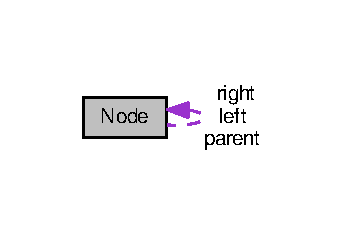
\includegraphics[width=160pt]{structNode__coll__graph}
\end{center}
\end{figure}
\subsection*{Public Attributes}
\begin{DoxyCompactItemize}
\item 
\mbox{\Hypertarget{structNode_ad88c9a757bfafd5ff265e0837b150056}\label{structNode_ad88c9a757bfafd5ff265e0837b150056}} 
char $\ast$ \hyperlink{structNode_ad88c9a757bfafd5ff265e0837b150056}{key}
\begin{DoxyCompactList}\small\item\em integer that represents a piece of data in the table (eg 35-\/$>$\char`\"{}hello\char`\"{}) \end{DoxyCompactList}\item 
\mbox{\Hypertarget{structNode_a38b733496e3eff5e0b4fcb11cd9b866a}\label{structNode_a38b733496e3eff5e0b4fcb11cd9b866a}} 
void $\ast$ \hyperlink{structNode_a38b733496e3eff5e0b4fcb11cd9b866a}{data}
\begin{DoxyCompactList}\small\item\em pointer to generic data that is to be stored in the hash table \end{DoxyCompactList}\item 
\mbox{\Hypertarget{structNode_af67b110ca1a258b793bf69d306929b22}\label{structNode_af67b110ca1a258b793bf69d306929b22}} 
struct \hyperlink{structNode}{Node} $\ast$ \hyperlink{structNode_af67b110ca1a258b793bf69d306929b22}{next}
\begin{DoxyCompactList}\small\item\em pointer to the next \hyperlink{structNode}{Node} if a collision is detected \end{DoxyCompactList}\end{DoxyCompactItemize}


\subsection{Detailed Description}
\hyperlink{structNode}{Node} of the hash table. 

The documentation for this struct was generated from the following file\+:\begin{DoxyCompactItemize}
\item 
include/\hyperlink{HashTableAPI_8h}{Hash\+Table\+A\+P\+I.\+h}\end{DoxyCompactItemize}

\chapter{File Documentation}
\hypertarget{heap_8h}{}\section{include/heap.h File Reference}
\label{heap_8h}\index{include/heap.\+h@{include/heap.\+h}}


File containing the function definitions of a heap.  


\subsection*{Macros}
\begin{DoxyCompactItemize}
\item 
\mbox{\Hypertarget{heap_8h_a4c6c6aff2b0e57a0ec4f2d4d6276a48d}\label{heap_8h_a4c6c6aff2b0e57a0ec4f2d4d6276a48d}} 
\#define {\bfseries M\+I\+N\+\_\+\+H\+E\+AP}~0
\item 
\mbox{\Hypertarget{heap_8h_abbeb121d44260375bbedb804aa56bdc0}\label{heap_8h_abbeb121d44260375bbedb804aa56bdc0}} 
\#define {\bfseries M\+A\+X\+\_\+\+H\+E\+AP}~1
\item 
\mbox{\Hypertarget{heap_8h_a3565d2f7ab5f5189c585448b1455fb09}\label{heap_8h_a3565d2f7ab5f5189c585448b1455fb09}} 
\#define {\bfseries H\+E\+A\+P\+\_\+\+T\+Y\+PE}~unsigned char
\end{DoxyCompactItemize}
\subsection*{Functions}
\begin{DoxyCompactItemize}
\item 
\hyperlink{structHeap}{Heap} $\ast$ \hyperlink{heap_8h_a7c03037ba44f097a29ba5ada3bb7e3cf}{create\+Heap} (size\+\_\+t initial\+Size, H\+E\+A\+P\+\_\+\+T\+Y\+PE htype, void($\ast$destroy\+Data\+FP)(void $\ast$data), void($\ast$print\+Node\+FP)(void $\ast$to\+Be\+Printed), int($\ast$compare\+FP)(const void $\ast$first, const void $\ast$second))
\item 
\hyperlink{structNode}{Node} $\ast$ \hyperlink{heap_8h_a8dfb88de5e4ff4d38e8510030373a6a4}{create\+Heap\+Node} (void $\ast$data)
\item 
void \hyperlink{heap_8h_a6aea510506dc9cf7255f37fdb69d6f4b}{insert\+Heap\+Node} (\hyperlink{structHeap}{Heap} $\ast$heap, void $\ast$data)
\item 
void \hyperlink{heap_8h_a812ef014f7e8c7567d6de69504a2f2af}{delete\+Min\+Or\+Max} (\hyperlink{structHeap}{Heap} $\ast$heap)
\item 
void $\ast$ \hyperlink{heap_8h_ad35b71ae5c43d7a26a577ee0d9297015}{get\+Min\+Or\+Max} (\hyperlink{structHeap}{Heap} $\ast$heap)
\item 
void \hyperlink{heap_8h_a20f07c1cc6a040fa62afffd83c2359b8}{change\+Heap\+Type} (\hyperlink{structHeap}{Heap} $\ast$heap)
\item 
void \hyperlink{heap_8h_ac0ddd1874bd4ad9992a3ab465a54dbbc}{delete\+Heap} (\hyperlink{structHeap}{Heap} $\ast$heap)
\end{DoxyCompactItemize}


\subsection{Detailed Description}
File containing the function definitions of a heap. 

\begin{DoxyAuthor}{Author}
Michael Ellis 
\end{DoxyAuthor}
\begin{DoxyDate}{Date}
March 2017 
\end{DoxyDate}


\subsection{Function Documentation}
\mbox{\Hypertarget{heap_8h_a20f07c1cc6a040fa62afffd83c2359b8}\label{heap_8h_a20f07c1cc6a040fa62afffd83c2359b8}} 
\index{heap.\+h@{heap.\+h}!change\+Heap\+Type@{change\+Heap\+Type}}
\index{change\+Heap\+Type@{change\+Heap\+Type}!heap.\+h@{heap.\+h}}
\subsubsection{\texorpdfstring{change\+Heap\+Type()}{changeHeapType()}}
{\footnotesize\ttfamily void change\+Heap\+Type (\begin{DoxyParamCaption}\item[{\hyperlink{structHeap}{Heap} $\ast$}]{heap }\end{DoxyParamCaption})}

Function to switch the type of heap from min-\/to-\/max or max-\/to-\/min. This changes the htype flag from M\+I\+N\+\_\+\+H\+E\+AP to M\+A\+X\+\_\+\+H\+E\+AP and vice versa. Once the flag has been changed, heapify is called on the heap to rearrange it to fit the new heap property. 
\begin{DoxyParams}{Parameters}
{\em heap} & Pointer to a heap to switch from min-\/to-\/max or max-\/to-\/min. \\
\hline
\end{DoxyParams}
\mbox{\Hypertarget{heap_8h_a7c03037ba44f097a29ba5ada3bb7e3cf}\label{heap_8h_a7c03037ba44f097a29ba5ada3bb7e3cf}} 
\index{heap.\+h@{heap.\+h}!create\+Heap@{create\+Heap}}
\index{create\+Heap@{create\+Heap}!heap.\+h@{heap.\+h}}
\subsubsection{\texorpdfstring{create\+Heap()}{createHeap()}}
{\footnotesize\ttfamily \hyperlink{structHeap}{Heap}$\ast$ create\+Heap (\begin{DoxyParamCaption}\item[{size\+\_\+t}]{initial\+Size,  }\item[{H\+E\+A\+P\+\_\+\+T\+Y\+PE}]{htype,  }\item[{void($\ast$)(void $\ast$data)}]{destroy\+Data\+FP,  }\item[{void($\ast$)(void $\ast$to\+Be\+Printed)}]{print\+Node\+FP,  }\item[{int($\ast$)(const void $\ast$first, const void $\ast$second)}]{compare\+FP }\end{DoxyParamCaption})}

Function to allocate memory to the heap and point the heap to the appropriate functions. Allocates memory to the heap based on the size given. \begin{DoxyReturn}{Returns}
pointer to the heap 
\end{DoxyReturn}

\begin{DoxyParams}{Parameters}
{\em initial\+Size} & initial size of the heap \\
\hline
{\em htype} & flag to choose whether to start the heap as a min heap or max heap. Takes in values M\+I\+N\+\_\+\+H\+E\+AP and M\+A\+X\+\_\+\+H\+E\+AP \\
\hline
{\em compare\+FP} & function pointer to a function that compares two pieces of data. \\
\hline
{\em destroy\+Data\+FP} & function pointer to a function to delete a single piece of data from the heap \\
\hline
{\em print\+Node\+FP} & function pointer to a function that prints out a data element of the heap \\
\hline
\end{DoxyParams}
\begin{DoxyReturn}{Returns}
pointer to the heap 
\end{DoxyReturn}
\mbox{\Hypertarget{heap_8h_a8dfb88de5e4ff4d38e8510030373a6a4}\label{heap_8h_a8dfb88de5e4ff4d38e8510030373a6a4}} 
\index{heap.\+h@{heap.\+h}!create\+Heap\+Node@{create\+Heap\+Node}}
\index{create\+Heap\+Node@{create\+Heap\+Node}!heap.\+h@{heap.\+h}}
\subsubsection{\texorpdfstring{create\+Heap\+Node()}{createHeapNode()}}
{\footnotesize\ttfamily \hyperlink{structNode}{Node}$\ast$ create\+Heap\+Node (\begin{DoxyParamCaption}\item[{void $\ast$}]{data }\end{DoxyParamCaption})}

Function for creating a node for a heap. \begin{DoxyPrecond}{Precondition}
\hyperlink{structNode}{Node} must be cast to void pointer before being added. 
\end{DoxyPrecond}
\begin{DoxyPostcond}{Postcondition}
\hyperlink{structNode}{Node} is valid and able to be added to a heap 
\end{DoxyPostcond}

\begin{DoxyParams}{Parameters}
{\em data} & is a generic pointer to any data type that is to be stored in the heap. \\
\hline
\end{DoxyParams}
\begin{DoxyReturn}{Returns}
returns a node for a heap 
\end{DoxyReturn}
\mbox{\Hypertarget{heap_8h_ac0ddd1874bd4ad9992a3ab465a54dbbc}\label{heap_8h_ac0ddd1874bd4ad9992a3ab465a54dbbc}} 
\index{heap.\+h@{heap.\+h}!delete\+Heap@{delete\+Heap}}
\index{delete\+Heap@{delete\+Heap}!heap.\+h@{heap.\+h}}
\subsubsection{\texorpdfstring{delete\+Heap()}{deleteHeap()}}
{\footnotesize\ttfamily void delete\+Heap (\begin{DoxyParamCaption}\item[{\hyperlink{structHeap}{Heap} $\ast$}]{heap }\end{DoxyParamCaption})}

Function delete a heap. This function calls delete\+Min\+Or\+Max the same amount of times as the size of the heap, which heapifies after each deletion. Finally, it frees the \hyperlink{structHeap}{Heap} structure. 
\begin{DoxyParams}{Parameters}
{\em heap} & Pointer of a heap to be deleted. \\
\hline
\end{DoxyParams}
\mbox{\Hypertarget{heap_8h_a812ef014f7e8c7567d6de69504a2f2af}\label{heap_8h_a812ef014f7e8c7567d6de69504a2f2af}} 
\index{heap.\+h@{heap.\+h}!delete\+Min\+Or\+Max@{delete\+Min\+Or\+Max}}
\index{delete\+Min\+Or\+Max@{delete\+Min\+Or\+Max}!heap.\+h@{heap.\+h}}
\subsubsection{\texorpdfstring{delete\+Min\+Or\+Max()}{deleteMinOrMax()}}
{\footnotesize\ttfamily void delete\+Min\+Or\+Max (\begin{DoxyParamCaption}\item[{\hyperlink{structHeap}{Heap} $\ast$}]{heap }\end{DoxyParamCaption})}

Function to remove the maximum or minimum \hyperlink{structNode}{Node} of the heap (depending on min heap or max heap). Once the \hyperlink{structNode}{Node} has been deleted, the \hyperlink{structNode}{Node} at the deepest point in the \hyperlink{structHeap}{Heap} is placed in the min/max position. Finally, the heap is heapified to maintain heap property. \begin{DoxyPrecond}{Precondition}
\hyperlink{structHeap}{Heap} must exist and have memory allocated to it 
\end{DoxyPrecond}

\begin{DoxyParams}{Parameters}
{\em heap} & Pointer to a heap. \\
\hline
\end{DoxyParams}
\mbox{\Hypertarget{heap_8h_ad35b71ae5c43d7a26a577ee0d9297015}\label{heap_8h_ad35b71ae5c43d7a26a577ee0d9297015}} 
\index{heap.\+h@{heap.\+h}!get\+Min\+Or\+Max@{get\+Min\+Or\+Max}}
\index{get\+Min\+Or\+Max@{get\+Min\+Or\+Max}!heap.\+h@{heap.\+h}}
\subsubsection{\texorpdfstring{get\+Min\+Or\+Max()}{getMinOrMax()}}
{\footnotesize\ttfamily void$\ast$ get\+Min\+Or\+Max (\begin{DoxyParamCaption}\item[{\hyperlink{structHeap}{Heap} $\ast$}]{heap }\end{DoxyParamCaption})}

Function to rearrange a heap to maintain heap property. Starting at the min/max, each \hyperlink{structNode}{Node} is compared with its two children to determine the smallest/largest of the three. If the parent is smaller/larger than the child, it is swapped. Heapify is then recursively called on the child in order to continue heapifying until it reaches the bottom of the heap. 
\begin{DoxyParams}{Parameters}
{\em heap} & Pointer to a heap to be heapified \\
\hline
\end{DoxyParams}
\mbox{\Hypertarget{heap_8h_a6aea510506dc9cf7255f37fdb69d6f4b}\label{heap_8h_a6aea510506dc9cf7255f37fdb69d6f4b}} 
\index{heap.\+h@{heap.\+h}!insert\+Heap\+Node@{insert\+Heap\+Node}}
\index{insert\+Heap\+Node@{insert\+Heap\+Node}!heap.\+h@{heap.\+h}}
\subsubsection{\texorpdfstring{insert\+Heap\+Node()}{insertHeapNode()}}
{\footnotesize\ttfamily void insert\+Heap\+Node (\begin{DoxyParamCaption}\item[{\hyperlink{structHeap}{Heap} $\ast$}]{heap,  }\item[{void $\ast$}]{data }\end{DoxyParamCaption})}

Inserts a \hyperlink{structNode}{Node} into the heap. Uses create\+Heap\+Node to place the data in a \hyperlink{structNode}{Node} structure, and then puts the newly created \hyperlink{structNode}{Node} in the heap by adding at the bottom and comparing it to each parent node until it fits the \hyperlink{structHeap}{Heap} structure. If the heap is a min heap, if the \hyperlink{structNode}{Node} is lesser than the parent, it is swapped. The opposite is true for a max heap. \begin{DoxyPrecond}{Precondition}
\hyperlink{structHeap}{Heap} must exist and have data allocated to it 
\end{DoxyPrecond}

\begin{DoxyParams}{Parameters}
{\em heap} & Pointer to a heap \\
\hline
{\em data} & Pointer to generic data that is to be inserted into the heap \\
\hline
\end{DoxyParams}

\hypertarget{heaphelper_8h}{}\section{include/heaphelper.h File Reference}
\label{heaphelper_8h}\index{include/heaphelper.\+h@{include/heaphelper.\+h}}


File containing the function definitions of a hash table.  


\subsection*{Classes}
\begin{DoxyCompactItemize}
\item 
struct \hyperlink{structNode}{Node}
\item 
struct \hyperlink{structHeap}{Heap}
\end{DoxyCompactItemize}
\subsection*{Macros}
\begin{DoxyCompactItemize}
\item 
\mbox{\Hypertarget{heaphelper_8h_a4c6c6aff2b0e57a0ec4f2d4d6276a48d}\label{heaphelper_8h_a4c6c6aff2b0e57a0ec4f2d4d6276a48d}} 
\#define {\bfseries M\+I\+N\+\_\+\+H\+E\+AP}~0
\item 
\mbox{\Hypertarget{heaphelper_8h_abbeb121d44260375bbedb804aa56bdc0}\label{heaphelper_8h_abbeb121d44260375bbedb804aa56bdc0}} 
\#define {\bfseries M\+A\+X\+\_\+\+H\+E\+AP}~1
\item 
\mbox{\Hypertarget{heaphelper_8h_a3565d2f7ab5f5189c585448b1455fb09}\label{heaphelper_8h_a3565d2f7ab5f5189c585448b1455fb09}} 
\#define {\bfseries H\+E\+A\+P\+\_\+\+T\+Y\+PE}~unsigned char
\end{DoxyCompactItemize}
\subsection*{Typedefs}
\begin{DoxyCompactItemize}
\item 
typedef struct \hyperlink{structNode}{Node} \hyperlink{heaphelper_8h_a3b09f37e675bcd48a01bf22155996872}{Node}
\item 
typedef struct \hyperlink{structHeap}{Heap} \hyperlink{heaphelper_8h_a705af815969c97892c0aaaa658f6c88c}{Heap}
\end{DoxyCompactItemize}
\subsection*{Functions}
\begin{DoxyCompactItemize}
\item 
void \hyperlink{heaphelper_8h_a1a636851e2018f56ce962313b4a9c06b}{heapify\+Up} (\hyperlink{structHeap}{Heap} $\ast$heap, \hyperlink{structNode}{Node} $\ast$node)
\item 
void \hyperlink{heaphelper_8h_af76c8147e0460cd6b03b3092940b619a}{heapify\+Down} (\hyperlink{structHeap}{Heap} $\ast$heap, \hyperlink{structNode}{Node} $\ast$node)
\item 
void \hyperlink{heaphelper_8h_aba460c46a38e2bae4dd2382fdc4f78e9}{print\+Heap} (\hyperlink{structHeap}{Heap} $\ast$heap)
\end{DoxyCompactItemize}


\subsection{Detailed Description}
File containing the function definitions of a hash table. 

\begin{DoxyAuthor}{Author}
Ralph Arvin De Castro 
\end{DoxyAuthor}
\begin{DoxyDate}{Date}
July 2018 
\end{DoxyDate}


\subsection{Typedef Documentation}
\mbox{\Hypertarget{heaphelper_8h_a705af815969c97892c0aaaa658f6c88c}\label{heaphelper_8h_a705af815969c97892c0aaaa658f6c88c}} 
\index{heaphelper.\+h@{heaphelper.\+h}!Heap@{Heap}}
\index{Heap@{Heap}!heaphelper.\+h@{heaphelper.\+h}}
\subsubsection{\texorpdfstring{Heap}{Heap}}
{\footnotesize\ttfamily typedef struct \hyperlink{structHeap}{Heap} \hyperlink{structHeap}{Heap}}

\hyperlink{structHeap}{Heap} structure for binary tree implementation of a \hyperlink{structHeap}{Heap} \mbox{\Hypertarget{heaphelper_8h_a3b09f37e675bcd48a01bf22155996872}\label{heaphelper_8h_a3b09f37e675bcd48a01bf22155996872}} 
\index{heaphelper.\+h@{heaphelper.\+h}!Node@{Node}}
\index{Node@{Node}!heaphelper.\+h@{heaphelper.\+h}}
\subsubsection{\texorpdfstring{Node}{Node}}
{\footnotesize\ttfamily typedef struct \hyperlink{structNode}{Node} \hyperlink{structNode}{Node}}

\hyperlink{structNode}{Node} of the heap 

\subsection{Function Documentation}
\mbox{\Hypertarget{heaphelper_8h_af76c8147e0460cd6b03b3092940b619a}\label{heaphelper_8h_af76c8147e0460cd6b03b3092940b619a}} 
\index{heaphelper.\+h@{heaphelper.\+h}!heapify\+Down@{heapify\+Down}}
\index{heapify\+Down@{heapify\+Down}!heaphelper.\+h@{heaphelper.\+h}}
\subsubsection{\texorpdfstring{heapify\+Down()}{heapifyDown()}}
{\footnotesize\ttfamily void heapify\+Down (\begin{DoxyParamCaption}\item[{\hyperlink{structHeap}{Heap} $\ast$}]{heap,  }\item[{\hyperlink{structNode}{Node} $\ast$}]{node }\end{DoxyParamCaption})}

Function to rearrange a heap to maintain heap property.\+Starts with a selected to heapify node then switch and traverse down if needed \begin{DoxyPrecond}{Precondition}
\hyperlink{structHeap}{Heap} must exist and have data allocated to it 
\end{DoxyPrecond}

\begin{DoxyParams}{Parameters}
{\em heap} & Pointer to a heap \\
\hline
{\em node} & Pointer to a node to heapify down \\
\hline
\end{DoxyParams}
\mbox{\Hypertarget{heaphelper_8h_a1a636851e2018f56ce962313b4a9c06b}\label{heaphelper_8h_a1a636851e2018f56ce962313b4a9c06b}} 
\index{heaphelper.\+h@{heaphelper.\+h}!heapify\+Up@{heapify\+Up}}
\index{heapify\+Up@{heapify\+Up}!heaphelper.\+h@{heaphelper.\+h}}
\subsubsection{\texorpdfstring{heapify\+Up()}{heapifyUp()}}
{\footnotesize\ttfamily void heapify\+Up (\begin{DoxyParamCaption}\item[{\hyperlink{structHeap}{Heap} $\ast$}]{heap,  }\item[{\hyperlink{structNode}{Node} $\ast$}]{node }\end{DoxyParamCaption})}

Function to rearrange a heap to maintain heap property.\+Starts with a selected to heapify node then switch and traverse up if needed \begin{DoxyPrecond}{Precondition}
\hyperlink{structHeap}{Heap} must exist and have data allocated to it 
\end{DoxyPrecond}

\begin{DoxyParams}{Parameters}
{\em heap} & Pointer to a heap \\
\hline
{\em node} & Pointer to a node to heapify up \\
\hline
\end{DoxyParams}
\mbox{\Hypertarget{heaphelper_8h_aba460c46a38e2bae4dd2382fdc4f78e9}\label{heaphelper_8h_aba460c46a38e2bae4dd2382fdc4f78e9}} 
\index{heaphelper.\+h@{heaphelper.\+h}!print\+Heap@{print\+Heap}}
\index{print\+Heap@{print\+Heap}!heaphelper.\+h@{heaphelper.\+h}}
\subsubsection{\texorpdfstring{print\+Heap()}{printHeap()}}
{\footnotesize\ttfamily void print\+Heap (\begin{DoxyParamCaption}\item[{\hyperlink{structHeap}{Heap} $\ast$}]{heap }\end{DoxyParamCaption})}

Function to print all the nodes of the heap \begin{DoxyPrecond}{Precondition}
\hyperlink{structHeap}{Heap} must exist and have data allocated to it 
\end{DoxyPrecond}

\begin{DoxyParams}{Parameters}
{\em heap} & Pointer to a heap \\
\hline
\end{DoxyParams}

%--- End generated contents ---

% Index
\backmatter
\newpage
\phantomsection
\clearemptydoublepage
\addcontentsline{toc}{chapter}{Index}
\printindex

\end{document}
